
% Default to the notebook output style

    


% Inherit from the specified cell style.




    
\documentclass[11pt]{article}

    
    
    \usepackage[T1]{fontenc}
    % Nicer default font (+ math font) than Computer Modern for most use cases
    \usepackage{mathpazo}

    % Basic figure setup, for now with no caption control since it's done
    % automatically by Pandoc (which extracts ![](path) syntax from Markdown).
    \usepackage{graphicx}
    % We will generate all images so they have a width \maxwidth. This means
    % that they will get their normal width if they fit onto the page, but
    % are scaled down if they would overflow the margins.
    \makeatletter
    \def\maxwidth{\ifdim\Gin@nat@width>\linewidth\linewidth
    \else\Gin@nat@width\fi}
    \makeatother
    \let\Oldincludegraphics\includegraphics
    % Set max figure width to be 80% of text width, for now hardcoded.
    \renewcommand{\includegraphics}[1]{\Oldincludegraphics[width=.8\maxwidth]{#1}}
    % Ensure that by default, figures have no caption (until we provide a
    % proper Figure object with a Caption API and a way to capture that
    % in the conversion process - todo).
    \usepackage{caption}
    \DeclareCaptionLabelFormat{nolabel}{}
    \captionsetup{labelformat=nolabel}

    \usepackage{adjustbox} % Used to constrain images to a maximum size 
    \usepackage{xcolor} % Allow colors to be defined
    \usepackage{enumerate} % Needed for markdown enumerations to work
    \usepackage{geometry} % Used to adjust the document margins
    \usepackage{amsmath} % Equations
    \usepackage{amssymb} % Equations
    \usepackage{textcomp} % defines textquotesingle
    % Hack from http://tex.stackexchange.com/a/47451/13684:
    \AtBeginDocument{%
        \def\PYZsq{\textquotesingle}% Upright quotes in Pygmentized code
    }
    \usepackage{upquote} % Upright quotes for verbatim code
    \usepackage{eurosym} % defines \euro
    \usepackage[mathletters]{ucs} % Extended unicode (utf-8) support
    \usepackage[utf8x]{inputenc} % Allow utf-8 characters in the tex document
    \usepackage{fancyvrb} % verbatim replacement that allows latex
    \usepackage{grffile} % extends the file name processing of package graphics 
                         % to support a larger range 
    % The hyperref package gives us a pdf with properly built
    % internal navigation ('pdf bookmarks' for the table of contents,
    % internal cross-reference links, web links for URLs, etc.)
    \usepackage{hyperref}
    \usepackage{longtable} % longtable support required by pandoc >1.10
    \usepackage{booktabs}  % table support for pandoc > 1.12.2
    \usepackage[inline]{enumitem} % IRkernel/repr support (it uses the enumerate* environment)
    \usepackage[normalem]{ulem} % ulem is needed to support strikethroughs (\sout)
                                % normalem makes italics be italics, not underlines
    

    
    
    % Colors for the hyperref package
    \definecolor{urlcolor}{rgb}{0,.145,.698}
    \definecolor{linkcolor}{rgb}{.71,0.21,0.01}
    \definecolor{citecolor}{rgb}{.12,.54,.11}

    % ANSI colors
    \definecolor{ansi-black}{HTML}{3E424D}
    \definecolor{ansi-black-intense}{HTML}{282C36}
    \definecolor{ansi-red}{HTML}{E75C58}
    \definecolor{ansi-red-intense}{HTML}{B22B31}
    \definecolor{ansi-green}{HTML}{00A250}
    \definecolor{ansi-green-intense}{HTML}{007427}
    \definecolor{ansi-yellow}{HTML}{DDB62B}
    \definecolor{ansi-yellow-intense}{HTML}{B27D12}
    \definecolor{ansi-blue}{HTML}{208FFB}
    \definecolor{ansi-blue-intense}{HTML}{0065CA}
    \definecolor{ansi-magenta}{HTML}{D160C4}
    \definecolor{ansi-magenta-intense}{HTML}{A03196}
    \definecolor{ansi-cyan}{HTML}{60C6C8}
    \definecolor{ansi-cyan-intense}{HTML}{258F8F}
    \definecolor{ansi-white}{HTML}{C5C1B4}
    \definecolor{ansi-white-intense}{HTML}{A1A6B2}

    % commands and environments needed by pandoc snippets
    % extracted from the output of `pandoc -s`
    \providecommand{\tightlist}{%
      \setlength{\itemsep}{0pt}\setlength{\parskip}{0pt}}
    \DefineVerbatimEnvironment{Highlighting}{Verbatim}{commandchars=\\\{\}}
    % Add ',fontsize=\small' for more characters per line
    \newenvironment{Shaded}{}{}
    \newcommand{\KeywordTok}[1]{\textcolor[rgb]{0.00,0.44,0.13}{\textbf{{#1}}}}
    \newcommand{\DataTypeTok}[1]{\textcolor[rgb]{0.56,0.13,0.00}{{#1}}}
    \newcommand{\DecValTok}[1]{\textcolor[rgb]{0.25,0.63,0.44}{{#1}}}
    \newcommand{\BaseNTok}[1]{\textcolor[rgb]{0.25,0.63,0.44}{{#1}}}
    \newcommand{\FloatTok}[1]{\textcolor[rgb]{0.25,0.63,0.44}{{#1}}}
    \newcommand{\CharTok}[1]{\textcolor[rgb]{0.25,0.44,0.63}{{#1}}}
    \newcommand{\StringTok}[1]{\textcolor[rgb]{0.25,0.44,0.63}{{#1}}}
    \newcommand{\CommentTok}[1]{\textcolor[rgb]{0.38,0.63,0.69}{\textit{{#1}}}}
    \newcommand{\OtherTok}[1]{\textcolor[rgb]{0.00,0.44,0.13}{{#1}}}
    \newcommand{\AlertTok}[1]{\textcolor[rgb]{1.00,0.00,0.00}{\textbf{{#1}}}}
    \newcommand{\FunctionTok}[1]{\textcolor[rgb]{0.02,0.16,0.49}{{#1}}}
    \newcommand{\RegionMarkerTok}[1]{{#1}}
    \newcommand{\ErrorTok}[1]{\textcolor[rgb]{1.00,0.00,0.00}{\textbf{{#1}}}}
    \newcommand{\NormalTok}[1]{{#1}}
    
    % Additional commands for more recent versions of Pandoc
    \newcommand{\ConstantTok}[1]{\textcolor[rgb]{0.53,0.00,0.00}{{#1}}}
    \newcommand{\SpecialCharTok}[1]{\textcolor[rgb]{0.25,0.44,0.63}{{#1}}}
    \newcommand{\VerbatimStringTok}[1]{\textcolor[rgb]{0.25,0.44,0.63}{{#1}}}
    \newcommand{\SpecialStringTok}[1]{\textcolor[rgb]{0.73,0.40,0.53}{{#1}}}
    \newcommand{\ImportTok}[1]{{#1}}
    \newcommand{\DocumentationTok}[1]{\textcolor[rgb]{0.73,0.13,0.13}{\textit{{#1}}}}
    \newcommand{\AnnotationTok}[1]{\textcolor[rgb]{0.38,0.63,0.69}{\textbf{\textit{{#1}}}}}
    \newcommand{\CommentVarTok}[1]{\textcolor[rgb]{0.38,0.63,0.69}{\textbf{\textit{{#1}}}}}
    \newcommand{\VariableTok}[1]{\textcolor[rgb]{0.10,0.09,0.49}{{#1}}}
    \newcommand{\ControlFlowTok}[1]{\textcolor[rgb]{0.00,0.44,0.13}{\textbf{{#1}}}}
    \newcommand{\OperatorTok}[1]{\textcolor[rgb]{0.40,0.40,0.40}{{#1}}}
    \newcommand{\BuiltInTok}[1]{{#1}}
    \newcommand{\ExtensionTok}[1]{{#1}}
    \newcommand{\PreprocessorTok}[1]{\textcolor[rgb]{0.74,0.48,0.00}{{#1}}}
    \newcommand{\AttributeTok}[1]{\textcolor[rgb]{0.49,0.56,0.16}{{#1}}}
    \newcommand{\InformationTok}[1]{\textcolor[rgb]{0.38,0.63,0.69}{\textbf{\textit{{#1}}}}}
    \newcommand{\WarningTok}[1]{\textcolor[rgb]{0.38,0.63,0.69}{\textbf{\textit{{#1}}}}}
    
    
    % Define a nice break command that doesn't care if a line doesn't already
    % exist.
    \def\br{\hspace*{\fill} \\* }
    % Math Jax compatability definitions
    \def\gt{>}
    \def\lt{<}
    % Document parameters
    \title{XOR Neural network}
    
    
    

    % Pygments definitions
    
\makeatletter
\def\PY@reset{\let\PY@it=\relax \let\PY@bf=\relax%
    \let\PY@ul=\relax \let\PY@tc=\relax%
    \let\PY@bc=\relax \let\PY@ff=\relax}
\def\PY@tok#1{\csname PY@tok@#1\endcsname}
\def\PY@toks#1+{\ifx\relax#1\empty\else%
    \PY@tok{#1}\expandafter\PY@toks\fi}
\def\PY@do#1{\PY@bc{\PY@tc{\PY@ul{%
    \PY@it{\PY@bf{\PY@ff{#1}}}}}}}
\def\PY#1#2{\PY@reset\PY@toks#1+\relax+\PY@do{#2}}

\expandafter\def\csname PY@tok@w\endcsname{\def\PY@tc##1{\textcolor[rgb]{0.73,0.73,0.73}{##1}}}
\expandafter\def\csname PY@tok@c\endcsname{\let\PY@it=\textit\def\PY@tc##1{\textcolor[rgb]{0.25,0.50,0.50}{##1}}}
\expandafter\def\csname PY@tok@cp\endcsname{\def\PY@tc##1{\textcolor[rgb]{0.74,0.48,0.00}{##1}}}
\expandafter\def\csname PY@tok@k\endcsname{\let\PY@bf=\textbf\def\PY@tc##1{\textcolor[rgb]{0.00,0.50,0.00}{##1}}}
\expandafter\def\csname PY@tok@kp\endcsname{\def\PY@tc##1{\textcolor[rgb]{0.00,0.50,0.00}{##1}}}
\expandafter\def\csname PY@tok@kt\endcsname{\def\PY@tc##1{\textcolor[rgb]{0.69,0.00,0.25}{##1}}}
\expandafter\def\csname PY@tok@o\endcsname{\def\PY@tc##1{\textcolor[rgb]{0.40,0.40,0.40}{##1}}}
\expandafter\def\csname PY@tok@ow\endcsname{\let\PY@bf=\textbf\def\PY@tc##1{\textcolor[rgb]{0.67,0.13,1.00}{##1}}}
\expandafter\def\csname PY@tok@nb\endcsname{\def\PY@tc##1{\textcolor[rgb]{0.00,0.50,0.00}{##1}}}
\expandafter\def\csname PY@tok@nf\endcsname{\def\PY@tc##1{\textcolor[rgb]{0.00,0.00,1.00}{##1}}}
\expandafter\def\csname PY@tok@nc\endcsname{\let\PY@bf=\textbf\def\PY@tc##1{\textcolor[rgb]{0.00,0.00,1.00}{##1}}}
\expandafter\def\csname PY@tok@nn\endcsname{\let\PY@bf=\textbf\def\PY@tc##1{\textcolor[rgb]{0.00,0.00,1.00}{##1}}}
\expandafter\def\csname PY@tok@ne\endcsname{\let\PY@bf=\textbf\def\PY@tc##1{\textcolor[rgb]{0.82,0.25,0.23}{##1}}}
\expandafter\def\csname PY@tok@nv\endcsname{\def\PY@tc##1{\textcolor[rgb]{0.10,0.09,0.49}{##1}}}
\expandafter\def\csname PY@tok@no\endcsname{\def\PY@tc##1{\textcolor[rgb]{0.53,0.00,0.00}{##1}}}
\expandafter\def\csname PY@tok@nl\endcsname{\def\PY@tc##1{\textcolor[rgb]{0.63,0.63,0.00}{##1}}}
\expandafter\def\csname PY@tok@ni\endcsname{\let\PY@bf=\textbf\def\PY@tc##1{\textcolor[rgb]{0.60,0.60,0.60}{##1}}}
\expandafter\def\csname PY@tok@na\endcsname{\def\PY@tc##1{\textcolor[rgb]{0.49,0.56,0.16}{##1}}}
\expandafter\def\csname PY@tok@nt\endcsname{\let\PY@bf=\textbf\def\PY@tc##1{\textcolor[rgb]{0.00,0.50,0.00}{##1}}}
\expandafter\def\csname PY@tok@nd\endcsname{\def\PY@tc##1{\textcolor[rgb]{0.67,0.13,1.00}{##1}}}
\expandafter\def\csname PY@tok@s\endcsname{\def\PY@tc##1{\textcolor[rgb]{0.73,0.13,0.13}{##1}}}
\expandafter\def\csname PY@tok@sd\endcsname{\let\PY@it=\textit\def\PY@tc##1{\textcolor[rgb]{0.73,0.13,0.13}{##1}}}
\expandafter\def\csname PY@tok@si\endcsname{\let\PY@bf=\textbf\def\PY@tc##1{\textcolor[rgb]{0.73,0.40,0.53}{##1}}}
\expandafter\def\csname PY@tok@se\endcsname{\let\PY@bf=\textbf\def\PY@tc##1{\textcolor[rgb]{0.73,0.40,0.13}{##1}}}
\expandafter\def\csname PY@tok@sr\endcsname{\def\PY@tc##1{\textcolor[rgb]{0.73,0.40,0.53}{##1}}}
\expandafter\def\csname PY@tok@ss\endcsname{\def\PY@tc##1{\textcolor[rgb]{0.10,0.09,0.49}{##1}}}
\expandafter\def\csname PY@tok@sx\endcsname{\def\PY@tc##1{\textcolor[rgb]{0.00,0.50,0.00}{##1}}}
\expandafter\def\csname PY@tok@m\endcsname{\def\PY@tc##1{\textcolor[rgb]{0.40,0.40,0.40}{##1}}}
\expandafter\def\csname PY@tok@gh\endcsname{\let\PY@bf=\textbf\def\PY@tc##1{\textcolor[rgb]{0.00,0.00,0.50}{##1}}}
\expandafter\def\csname PY@tok@gu\endcsname{\let\PY@bf=\textbf\def\PY@tc##1{\textcolor[rgb]{0.50,0.00,0.50}{##1}}}
\expandafter\def\csname PY@tok@gd\endcsname{\def\PY@tc##1{\textcolor[rgb]{0.63,0.00,0.00}{##1}}}
\expandafter\def\csname PY@tok@gi\endcsname{\def\PY@tc##1{\textcolor[rgb]{0.00,0.63,0.00}{##1}}}
\expandafter\def\csname PY@tok@gr\endcsname{\def\PY@tc##1{\textcolor[rgb]{1.00,0.00,0.00}{##1}}}
\expandafter\def\csname PY@tok@ge\endcsname{\let\PY@it=\textit}
\expandafter\def\csname PY@tok@gs\endcsname{\let\PY@bf=\textbf}
\expandafter\def\csname PY@tok@gp\endcsname{\let\PY@bf=\textbf\def\PY@tc##1{\textcolor[rgb]{0.00,0.00,0.50}{##1}}}
\expandafter\def\csname PY@tok@go\endcsname{\def\PY@tc##1{\textcolor[rgb]{0.53,0.53,0.53}{##1}}}
\expandafter\def\csname PY@tok@gt\endcsname{\def\PY@tc##1{\textcolor[rgb]{0.00,0.27,0.87}{##1}}}
\expandafter\def\csname PY@tok@err\endcsname{\def\PY@bc##1{\setlength{\fboxsep}{0pt}\fcolorbox[rgb]{1.00,0.00,0.00}{1,1,1}{\strut ##1}}}
\expandafter\def\csname PY@tok@kc\endcsname{\let\PY@bf=\textbf\def\PY@tc##1{\textcolor[rgb]{0.00,0.50,0.00}{##1}}}
\expandafter\def\csname PY@tok@kd\endcsname{\let\PY@bf=\textbf\def\PY@tc##1{\textcolor[rgb]{0.00,0.50,0.00}{##1}}}
\expandafter\def\csname PY@tok@kn\endcsname{\let\PY@bf=\textbf\def\PY@tc##1{\textcolor[rgb]{0.00,0.50,0.00}{##1}}}
\expandafter\def\csname PY@tok@kr\endcsname{\let\PY@bf=\textbf\def\PY@tc##1{\textcolor[rgb]{0.00,0.50,0.00}{##1}}}
\expandafter\def\csname PY@tok@bp\endcsname{\def\PY@tc##1{\textcolor[rgb]{0.00,0.50,0.00}{##1}}}
\expandafter\def\csname PY@tok@fm\endcsname{\def\PY@tc##1{\textcolor[rgb]{0.00,0.00,1.00}{##1}}}
\expandafter\def\csname PY@tok@vc\endcsname{\def\PY@tc##1{\textcolor[rgb]{0.10,0.09,0.49}{##1}}}
\expandafter\def\csname PY@tok@vg\endcsname{\def\PY@tc##1{\textcolor[rgb]{0.10,0.09,0.49}{##1}}}
\expandafter\def\csname PY@tok@vi\endcsname{\def\PY@tc##1{\textcolor[rgb]{0.10,0.09,0.49}{##1}}}
\expandafter\def\csname PY@tok@vm\endcsname{\def\PY@tc##1{\textcolor[rgb]{0.10,0.09,0.49}{##1}}}
\expandafter\def\csname PY@tok@sa\endcsname{\def\PY@tc##1{\textcolor[rgb]{0.73,0.13,0.13}{##1}}}
\expandafter\def\csname PY@tok@sb\endcsname{\def\PY@tc##1{\textcolor[rgb]{0.73,0.13,0.13}{##1}}}
\expandafter\def\csname PY@tok@sc\endcsname{\def\PY@tc##1{\textcolor[rgb]{0.73,0.13,0.13}{##1}}}
\expandafter\def\csname PY@tok@dl\endcsname{\def\PY@tc##1{\textcolor[rgb]{0.73,0.13,0.13}{##1}}}
\expandafter\def\csname PY@tok@s2\endcsname{\def\PY@tc##1{\textcolor[rgb]{0.73,0.13,0.13}{##1}}}
\expandafter\def\csname PY@tok@sh\endcsname{\def\PY@tc##1{\textcolor[rgb]{0.73,0.13,0.13}{##1}}}
\expandafter\def\csname PY@tok@s1\endcsname{\def\PY@tc##1{\textcolor[rgb]{0.73,0.13,0.13}{##1}}}
\expandafter\def\csname PY@tok@mb\endcsname{\def\PY@tc##1{\textcolor[rgb]{0.40,0.40,0.40}{##1}}}
\expandafter\def\csname PY@tok@mf\endcsname{\def\PY@tc##1{\textcolor[rgb]{0.40,0.40,0.40}{##1}}}
\expandafter\def\csname PY@tok@mh\endcsname{\def\PY@tc##1{\textcolor[rgb]{0.40,0.40,0.40}{##1}}}
\expandafter\def\csname PY@tok@mi\endcsname{\def\PY@tc##1{\textcolor[rgb]{0.40,0.40,0.40}{##1}}}
\expandafter\def\csname PY@tok@il\endcsname{\def\PY@tc##1{\textcolor[rgb]{0.40,0.40,0.40}{##1}}}
\expandafter\def\csname PY@tok@mo\endcsname{\def\PY@tc##1{\textcolor[rgb]{0.40,0.40,0.40}{##1}}}
\expandafter\def\csname PY@tok@ch\endcsname{\let\PY@it=\textit\def\PY@tc##1{\textcolor[rgb]{0.25,0.50,0.50}{##1}}}
\expandafter\def\csname PY@tok@cm\endcsname{\let\PY@it=\textit\def\PY@tc##1{\textcolor[rgb]{0.25,0.50,0.50}{##1}}}
\expandafter\def\csname PY@tok@cpf\endcsname{\let\PY@it=\textit\def\PY@tc##1{\textcolor[rgb]{0.25,0.50,0.50}{##1}}}
\expandafter\def\csname PY@tok@c1\endcsname{\let\PY@it=\textit\def\PY@tc##1{\textcolor[rgb]{0.25,0.50,0.50}{##1}}}
\expandafter\def\csname PY@tok@cs\endcsname{\let\PY@it=\textit\def\PY@tc##1{\textcolor[rgb]{0.25,0.50,0.50}{##1}}}

\def\PYZbs{\char`\\}
\def\PYZus{\char`\_}
\def\PYZob{\char`\{}
\def\PYZcb{\char`\}}
\def\PYZca{\char`\^}
\def\PYZam{\char`\&}
\def\PYZlt{\char`\<}
\def\PYZgt{\char`\>}
\def\PYZsh{\char`\#}
\def\PYZpc{\char`\%}
\def\PYZdl{\char`\$}
\def\PYZhy{\char`\-}
\def\PYZsq{\char`\'}
\def\PYZdq{\char`\"}
\def\PYZti{\char`\~}
% for compatibility with earlier versions
\def\PYZat{@}
\def\PYZlb{[}
\def\PYZrb{]}
\makeatother


    % Exact colors from NB
    \definecolor{incolor}{rgb}{0.0, 0.0, 0.5}
    \definecolor{outcolor}{rgb}{0.545, 0.0, 0.0}



    
    % Prevent overflowing lines due to hard-to-break entities
    \sloppy 
    % Setup hyperref package
    \hypersetup{
      breaklinks=true,  % so long urls are correctly broken across lines
      colorlinks=true,
      urlcolor=urlcolor,
      linkcolor=linkcolor,
      citecolor=citecolor,
      }
    % Slightly bigger margins than the latex defaults
    
    \geometry{verbose,tmargin=1in,bmargin=1in,lmargin=1in,rmargin=1in}
    
    

    \begin{document}
    
    
    \maketitle
    
    

    
    \section{Simple Neural Network using Tensorflow for solving XOR
function}\label{simple-neural-network-using-tensorflow-for-solving-xor-function}

** Introduction : ** In this notebook we will go through the steps of
making a simple 2-layer neural network that will learn the XOR function.
The XOR function, exclusive or, will give us a 1 only if one of the
inputs is zero and the other one, in cases of both beeing one or zero it
returns zero, as can be seen in the following table. Where x1 and x2 are
the inputs to the function and Y the output. We will use this data to
train our model on as these cover all the usecases for the function.

\begin{longtable}[]{@{}ccc@{}}
\toprule
x1 & x2 & Y\tabularnewline
\midrule
\endhead
0 & 0 & 0\tabularnewline
0 & 1 & 1\tabularnewline
1 & 0 & 1\tabularnewline
1 & 1 & 0\tabularnewline
\bottomrule
\end{longtable}

** Implementation : ** To start building the model we will use for this
function we will first import the following packages:

\begin{itemize}
\tightlist
\item
  Tensorflow
\item
  Numpy
\end{itemize}

    \begin{Verbatim}[commandchars=\\\{\}]
{\color{incolor}In [{\color{incolor}11}]:} \PY{o}{\PYZpc{}}\PY{k}{matplotlib} inline
         \PY{k+kn}{import} \PY{n+nn}{numpy} \PY{k}{as} \PY{n+nn}{np}
         \PY{k+kn}{import} \PY{n+nn}{tensorflow} \PY{k}{as} \PY{n+nn}{tf}
         \PY{k+kn}{import} \PY{n+nn}{matplotlib}\PY{n+nn}{.}\PY{n+nn}{pyplot} \PY{k}{as} \PY{n+nn}{plt}
         
         \PY{c+c1}{\PYZsh{} Training data as presented in the table above}
         
         \PY{n}{X\PYZus{}train} \PY{o}{=} \PY{n}{np}\PY{o}{.}\PY{n}{array}\PY{p}{(}\PY{p}{[}\PY{p}{[}\PY{l+m+mf}{0.}\PY{p}{,} \PY{l+m+mf}{0.}\PY{p}{]}\PY{p}{,} \PY{p}{[}\PY{l+m+mf}{0.}\PY{p}{,} \PY{l+m+mf}{1.}\PY{p}{]}\PY{p}{,} \PY{p}{[}\PY{l+m+mf}{1.}\PY{p}{,} \PY{l+m+mf}{0.}\PY{p}{]}\PY{p}{,} \PY{p}{[}\PY{l+m+mf}{1.}\PY{p}{,} \PY{l+m+mf}{1.}\PY{p}{]}\PY{p}{]}\PY{p}{,} \PY{n}{dtype}\PY{o}{=}\PY{n}{np}\PY{o}{.}\PY{n}{float32}\PY{p}{)}
         \PY{n}{Y\PYZus{}train} \PY{o}{=} \PY{n}{np}\PY{o}{.}\PY{n}{array}\PY{p}{(}\PY{p}{[}\PY{p}{[}\PY{l+m+mf}{0.}\PY{p}{]}\PY{p}{,} \PY{p}{[}\PY{l+m+mf}{1.}\PY{p}{]}\PY{p}{,} \PY{p}{[}\PY{l+m+mf}{1.}\PY{p}{]}\PY{p}{,} \PY{p}{[}\PY{l+m+mf}{0.}\PY{p}{]}\PY{p}{]}\PY{p}{,} \PY{n}{dtype}\PY{o}{=}\PY{n}{np}\PY{o}{.}\PY{n}{float32}\PY{p}{)}
\end{Verbatim}


    We will use the Interactive Session from Tensorflow so that the Session
is implicitly part of any call to \(eval()\), that way we dont have to
pass the Session variable around making the code easier to read.

    \begin{Verbatim}[commandchars=\\\{\}]
{\color{incolor}In [{\color{incolor}12}]:} \PY{n}{sess} \PY{o}{=} \PY{n}{tf}\PY{o}{.}\PY{n}{InteractiveSession}\PY{p}{(}\PY{p}{)}
\end{Verbatim}


    \subsubsection{Model}\label{model}

The neural network model we will be building will be a two layer neural
network. Which we can see in the following figure :

\begin{figure}
\centering
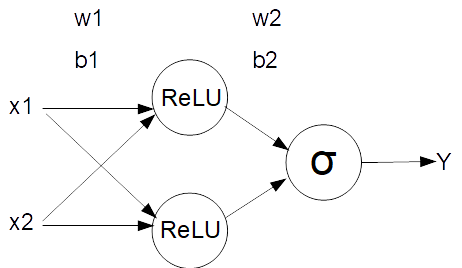
\includegraphics{nn_model.png}
\caption{Figure 1.) Neural network structure}
\end{figure}

As we can see from the figure above, the activation function for the
hidden layer will be the
\href{https://medium.com/tinymind/a-practical-guide-to-relu-b83ca804f1f7}{ReLU}
(rectified linear unit) function and for the output layer we will be
using the \href{https://en.wikipedia.org/wiki/Sigmoid_function}{Sigmoid}
activation.

To start building the neural network we will first have to define the
variables for the weights \(w1\), \(w2\) and biases \(b1\), \(b2\). As
we can see from the model structure above the model will have 2 input
features \(x1\) and \(x2\), with :

\begin{itemize}
\tightlist
\item
  \(n_{in}\) ... number of input features
\item
  \(n_{hidd}\) ... number of nodes in hidden layer
\end{itemize}

The weight matrices and bias vectors will have the following shapes :

\begin{itemize}
\tightlist
\item
  \(w_1.shape = (n_{in},n_{hidd})\)
\item
  \(b_1.shape = (1,n_{hidd})\)
\item
  \(w_2.shape = (n_{hidd},1)\)
\item
  \(b_2.shape = (1,1)\)
\end{itemize}

To implement this using tensorflow you can use this code :

    \begin{Verbatim}[commandchars=\\\{\}]
{\color{incolor}In [{\color{incolor}13}]:} \PY{n}{n\PYZus{}in} \PY{o}{=} \PY{l+m+mi}{2}
         \PY{n}{n\PYZus{}hidd} \PY{o}{=} \PY{l+m+mi}{2}
         
         \PY{n}{w1} \PY{o}{=} \PY{n}{tf}\PY{o}{.}\PY{n}{Variable}\PY{p}{(}\PY{n}{tf}\PY{o}{.}\PY{n}{random\PYZus{}uniform}\PY{p}{(}\PY{p}{[}\PY{n}{n\PYZus{}in}\PY{p}{,} \PY{n}{n\PYZus{}hidd}\PY{p}{]}\PY{p}{,} \PY{o}{\PYZhy{}}\PY{l+m+mi}{1}\PY{p}{,} \PY{l+m+mi}{1}\PY{p}{)}\PY{p}{,} \PY{n}{trainable}\PY{o}{=}\PY{k+kc}{True}\PY{p}{)}
         \PY{n}{b1} \PY{o}{=} \PY{n}{tf}\PY{o}{.}\PY{n}{Variable}\PY{p}{(}\PY{n}{tf}\PY{o}{.}\PY{n}{zeros}\PY{p}{(}\PY{n}{n\PYZus{}hidd}\PY{p}{)}\PY{p}{)}
         \PY{n}{w2} \PY{o}{=} \PY{n}{tf}\PY{o}{.}\PY{n}{Variable}\PY{p}{(}\PY{n}{tf}\PY{o}{.}\PY{n}{random\PYZus{}uniform}\PY{p}{(}\PY{p}{[}\PY{n}{n\PYZus{}hidd}\PY{p}{,} \PY{l+m+mi}{1}\PY{p}{]}\PY{p}{,} \PY{o}{\PYZhy{}}\PY{l+m+mi}{1}\PY{p}{,} \PY{l+m+mi}{1}\PY{p}{)}\PY{p}{,} \PY{n}{trainable}\PY{o}{=}\PY{k+kc}{True}\PY{p}{)}
         \PY{n}{b2} \PY{o}{=} \PY{n}{tf}\PY{o}{.}\PY{n}{Variable}\PY{p}{(}\PY{n}{tf}\PY{o}{.}\PY{n}{zeros}\PY{p}{(}\PY{l+m+mi}{1}\PY{p}{)}\PY{p}{)}
\end{Verbatim}


    The next step is to define a so called \emph{placeholder} using
tensorflow for the input vector, \(x\), and a \emph{placeholder} for the
true label vector, \(y\), which will be used for computing the cost. The
difference between variables and placeholders in tensorflow is that
variables need to be initialized by the session before they're used,
whereas placeholders are initialized by the session wherever they are
run. We define them as follows :

    \begin{Verbatim}[commandchars=\\\{\}]
{\color{incolor}In [{\color{incolor}14}]:} \PY{n}{x} \PY{o}{=} \PY{n}{tf}\PY{o}{.}\PY{n}{placeholder}\PY{p}{(}\PY{n}{shape}\PY{o}{=}\PY{p}{(}\PY{k+kc}{None}\PY{p}{,} \PY{n}{n\PYZus{}in}\PY{p}{)}\PY{p}{,} \PY{n}{dtype}\PY{o}{=}\PY{n}{tf}\PY{o}{.}\PY{n}{float32}\PY{p}{)} 
         \PY{n}{y} \PY{o}{=} \PY{n}{tf}\PY{o}{.}\PY{n}{placeholder}\PY{p}{(}\PY{n}{shape}\PY{o}{=}\PY{p}{(}\PY{k+kc}{None}\PY{p}{,} \PY{l+m+mi}{1}\PY{p}{)}\PY{p}{,} \PY{n}{dtype}\PY{o}{=}\PY{n}{tf}\PY{o}{.}\PY{n}{float32}\PY{p}{)}
\end{Verbatim}


    Now we can use the previously defined blocks and start adding them
together to build the model presented earlier.

To feed the input features to the hidden layer nodes and then to the
output layer we will use the following equations :

\[z_1 = w_1^Tx + b_1\] \[a_1 = relu(z_1)\] \[z_2 = w_2^Tx + b_2\]
\[a_2 = \sigma(z_2)\]

In the above equations we have implemented the activation functions as
presented in Figure 1., the tensorflow code :

    \begin{Verbatim}[commandchars=\\\{\}]
{\color{incolor}In [{\color{incolor}15}]:} \PY{n}{z1} \PY{o}{=} \PY{n}{tf}\PY{o}{.}\PY{n}{matmul}\PY{p}{(}\PY{n}{x}\PY{p}{,} \PY{n}{w1}\PY{p}{)} \PY{o}{+} \PY{n}{b1}
         \PY{n}{a1} \PY{o}{=} \PY{n}{tf}\PY{o}{.}\PY{n}{nn}\PY{o}{.}\PY{n}{relu}\PY{p}{(}\PY{n}{z1}\PY{p}{)}
         \PY{n}{z2} \PY{o}{=} \PY{n}{tf}\PY{o}{.}\PY{n}{matmul}\PY{p}{(}\PY{n}{a1}\PY{p}{,} \PY{n}{w2}\PY{p}{)} \PY{o}{+} \PY{n}{b2}
         \PY{n}{a2} \PY{o}{=} \PY{n}{tf}\PY{o}{.}\PY{n}{sigmoid}\PY{p}{(}\PY{n}{z2}\PY{p}{)}
\end{Verbatim}


    We have now completed the forward propagation implementation part of the
neural network model. Implementing the cost function and gradient
descent, where the learning happens, is the next step. Doing so is
pretty easy with tensorflow but reading up on
\href{https://hackernoon.com/gradient-descent-aynk-7cbe95a778da}{gradient
descent} and coding it yourself would be a very good exercise and is
highly recommended. Regarding the gradient descent we need to choose a
good learning rate, we will use \(0.1\) but you should also try smaller
and bigger values to see how the model evolves.

As our loss we will implement the following function :

\[J = -(y \cdot log(a2) + (1 - y) \cdot log(1 - a2))\]

And use the gradient descent algorithm to minimize the cost computed
over our training examples. To rule out any missconceptions, "loss" is
used when reffering to a single training example and the "cost" is over
the entire training set. The tensorflow code for the loss and gradient
descent is :

    \begin{Verbatim}[commandchars=\\\{\}]
{\color{incolor}In [{\color{incolor}36}]:} \PY{n}{learning\PYZus{}rate} \PY{o}{=} \PY{l+m+mf}{0.1}
         \PY{n}{cost} \PY{o}{=} \PY{n}{tf}\PY{o}{.}\PY{n}{reduce\PYZus{}mean}\PY{p}{(}\PY{o}{\PYZhy{}}\PY{p}{(}\PY{n}{y}\PY{o}{*}\PY{n}{tf}\PY{o}{.}\PY{n}{log}\PY{p}{(}\PY{n}{a2}\PY{p}{)} \PY{o}{+} \PY{p}{(}\PY{l+m+mi}{1}\PY{o}{\PYZhy{}}\PY{n}{y}\PY{p}{)}\PY{o}{*}\PY{n}{tf}\PY{o}{.}\PY{n}{log}\PY{p}{(}\PY{l+m+mi}{1}\PY{o}{\PYZhy{}}\PY{n}{a2}\PY{p}{)}\PY{p}{)}\PY{p}{)} 
         \PY{n}{train\PYZus{}step} \PY{o}{=} \PY{n}{tf}\PY{o}{.}\PY{n}{train}\PY{o}{.}\PY{n}{GradientDescentOptimizer}\PY{p}{(}\PY{n}{learning\PYZus{}rate}\PY{p}{)}\PY{o}{.}\PY{n}{minimize}\PY{p}{(}\PY{n}{cost}\PY{p}{)}
\end{Verbatim}


    In this step we will have to define a variable initializer which will
initialize all the variables defined earlier so that they can be used
properly by the code we wrote previously. An important note here is that
depending on the initialized values for the weights you will be able to
observe the cost converging to a relatively high value and staying
around that point or you will see the cost converging rapidly to a value
close to zero. So if you get a slow convergence first time running, try
it again until you hit initial values that allow a much faster
convergence.

Now we will just need to repeat the gradient descent for a number of
iterations, in our case we will run the training for \(20000\)
iterations and print the cost every \(1000\) iterations.

    \begin{Verbatim}[commandchars=\\\{\}]
{\color{incolor}In [{\color{incolor}37}]:} \PY{c+c1}{\PYZsh{} simple function for calculating the accuracy}
         
         \PY{k}{def} \PY{n+nf}{calc\PYZus{}acc}\PY{p}{(}\PY{n}{y1}\PY{p}{,} \PY{n}{y2}\PY{p}{)}\PY{p}{:}
             \PY{n}{miss} \PY{o}{=} \PY{l+m+mi}{0}
             \PY{k}{for} \PY{n}{v1}\PY{p}{,}\PY{n}{v2} \PY{o+ow}{in} \PY{n+nb}{zip}\PY{p}{(}\PY{n}{y1}\PY{p}{,}\PY{n}{y2}\PY{p}{)}\PY{p}{:}
                 \PY{k}{if} \PY{n}{v1} \PY{o}{!=} \PY{n}{v2}\PY{p}{:}
                     \PY{n}{miss} \PY{o}{+}\PY{o}{=} \PY{l+m+mi}{1}
             \PY{k}{return} \PY{p}{(}\PY{p}{(}\PY{n+nb}{len}\PY{p}{(}\PY{n}{y1}\PY{p}{)}\PY{o}{\PYZhy{}}\PY{n}{miss}\PY{p}{)}\PY{o}{/}\PY{n+nb}{len}\PY{p}{(}\PY{n}{y1}\PY{p}{)}\PY{p}{)}\PY{o}{*}\PY{l+m+mi}{100}
\end{Verbatim}


    \begin{Verbatim}[commandchars=\\\{\}]
{\color{incolor}In [{\color{incolor}38}]:} \PY{n}{init} \PY{o}{=} \PY{n}{tf}\PY{o}{.}\PY{n}{global\PYZus{}variables\PYZus{}initializer}\PY{p}{(}\PY{p}{)}
         \PY{n}{init}\PY{o}{.}\PY{n}{run}\PY{p}{(}\PY{p}{)}
         
         \PY{n}{cost\PYZus{}list} \PY{o}{=} \PY{p}{[}\PY{p}{]}
         \PY{n}{acc\PYZus{}list} \PY{o}{=} \PY{p}{[}\PY{p}{]}
         \PY{k}{for} \PY{n}{i} \PY{o+ow}{in} \PY{n+nb}{range}\PY{p}{(}\PY{l+m+mi}{20000}\PY{p}{)}\PY{p}{:}
             \PY{n}{train\PYZus{}step}\PY{o}{.}\PY{n}{run}\PY{p}{(}\PY{n}{feed\PYZus{}dict}\PY{o}{=}\PY{p}{\PYZob{}}\PY{n}{x}\PY{p}{:} \PY{n}{X\PYZus{}train}\PY{p}{,} \PY{n}{y}\PY{p}{:} \PY{n}{Y\PYZus{}train}\PY{p}{\PYZcb{}}\PY{p}{)}
             \PY{k}{if} \PY{n}{i}\PY{o}{\PYZpc{}}\PY{k}{1000} == 0:
                 \PY{n}{curr\PYZus{}cost} \PY{o}{=} \PY{n}{cost}\PY{o}{.}\PY{n}{eval}\PY{p}{(}\PY{n}{feed\PYZus{}dict}\PY{o}{=}\PY{p}{\PYZob{}}\PY{n}{x}\PY{p}{:} \PY{n}{X\PYZus{}train}\PY{p}{,} \PY{n}{y}\PY{p}{:} \PY{n}{Y\PYZus{}train}\PY{p}{\PYZcb{}}\PY{p}{)}
                 \PY{n}{y\PYZus{}pred} \PY{o}{=} \PY{n}{a2}\PY{o}{.}\PY{n}{eval}\PY{p}{(}\PY{n}{feed\PYZus{}dict}\PY{o}{=}\PY{p}{\PYZob{}}\PY{n}{x}\PY{p}{:} \PY{n}{X\PYZus{}train}\PY{p}{\PYZcb{}}\PY{p}{)}
                 \PY{n}{y\PYZus{}pred} \PY{o}{=} \PY{p}{(}\PY{n}{y\PYZus{}pred} \PY{o}{\PYZgt{}} \PY{l+m+mf}{0.5}\PY{p}{)}\PY{o}{.}\PY{n}{astype}\PY{p}{(}\PY{n}{np}\PY{o}{.}\PY{n}{float32}\PY{p}{)}
                 \PY{n}{curr\PYZus{}acc} \PY{o}{=} \PY{n}{calc\PYZus{}acc}\PY{p}{(}\PY{n}{Y\PYZus{}train}\PY{p}{,} \PY{n}{y\PYZus{}pred}\PY{p}{)}
                 \PY{n+nb}{print}\PY{p}{(}\PY{l+s+s1}{\PYZsq{}}\PY{l+s+s1}{Iter = }\PY{l+s+si}{\PYZob{}\PYZcb{}}\PY{l+s+s1}{, Cost = }\PY{l+s+si}{\PYZob{}:.3f\PYZcb{}}\PY{l+s+s1}{, Acc = }\PY{l+s+si}{\PYZob{}:.2f\PYZcb{}}\PY{l+s+s1}{\PYZpc{}}\PY{l+s+s1}{\PYZsq{}}\PY{o}{.}\PY{n}{format}\PY{p}{(}\PY{n}{i}\PY{p}{,} \PY{n}{curr\PYZus{}cost}\PY{p}{,} \PY{n}{curr\PYZus{}acc}\PY{p}{)}\PY{p}{)}
                 \PY{n}{cost\PYZus{}list}\PY{o}{.}\PY{n}{append}\PY{p}{(}\PY{n}{curr\PYZus{}cost}\PY{p}{)}
                 \PY{n}{acc\PYZus{}list}\PY{o}{.}\PY{n}{append}\PY{p}{(}\PY{n}{curr\PYZus{}acc}\PY{p}{)}
                 
         \PY{n}{plt}\PY{o}{.}\PY{n}{plot}\PY{p}{(}\PY{n}{cost\PYZus{}list}\PY{p}{)}
         \PY{n}{plt}\PY{o}{.}\PY{n}{ylabel}\PY{p}{(}\PY{l+s+s1}{\PYZsq{}}\PY{l+s+s1}{Cost}\PY{l+s+s1}{\PYZsq{}}\PY{p}{)}
         \PY{n}{plt}\PY{o}{.}\PY{n}{xlabel}\PY{p}{(}\PY{l+s+s1}{\PYZsq{}}\PY{l+s+s1}{iterations (per thousands)}\PY{l+s+s1}{\PYZsq{}}\PY{p}{)}
         \PY{n}{plt}\PY{o}{.}\PY{n}{title}\PY{p}{(}\PY{l+s+s2}{\PYZdq{}}\PY{l+s+s2}{Learning rate =}\PY{l+s+s2}{\PYZdq{}} \PY{o}{+} \PY{n+nb}{str}\PY{p}{(}\PY{n}{learning\PYZus{}rate}\PY{p}{)}\PY{p}{)}
         \PY{n}{plt}\PY{o}{.}\PY{n}{show}\PY{p}{(}\PY{p}{)}
         
         \PY{n}{plt}\PY{o}{.}\PY{n}{plot}\PY{p}{(}\PY{n}{acc\PYZus{}list}\PY{p}{)}
         \PY{n}{plt}\PY{o}{.}\PY{n}{ylabel}\PY{p}{(}\PY{l+s+s1}{\PYZsq{}}\PY{l+s+s1}{Accuracy [}\PY{l+s+s1}{\PYZpc{}}\PY{l+s+s1}{]}\PY{l+s+s1}{\PYZsq{}}\PY{p}{)}
         \PY{n}{plt}\PY{o}{.}\PY{n}{xlabel}\PY{p}{(}\PY{l+s+s1}{\PYZsq{}}\PY{l+s+s1}{iterations (per thousands)}\PY{l+s+s1}{\PYZsq{}}\PY{p}{)}
         \PY{n}{plt}\PY{o}{.}\PY{n}{title}\PY{p}{(}\PY{l+s+s2}{\PYZdq{}}\PY{l+s+s2}{Learning rate =}\PY{l+s+s2}{\PYZdq{}} \PY{o}{+} \PY{n+nb}{str}\PY{p}{(}\PY{n}{learning\PYZus{}rate}\PY{p}{)}\PY{p}{)}
         \PY{n}{plt}\PY{o}{.}\PY{n}{show}\PY{p}{(}\PY{p}{)}
\end{Verbatim}


    \begin{Verbatim}[commandchars=\\\{\}]
Iter = 0, Cost = 0.644, Acc = 50.00\%
Iter = 1000, Cost = 0.030, Acc = 100.00\%
Iter = 2000, Cost = 0.011, Acc = 100.00\%
Iter = 3000, Cost = 0.006, Acc = 100.00\%
Iter = 4000, Cost = 0.004, Acc = 100.00\%
Iter = 5000, Cost = 0.003, Acc = 100.00\%
Iter = 6000, Cost = 0.003, Acc = 100.00\%
Iter = 7000, Cost = 0.002, Acc = 100.00\%
Iter = 8000, Cost = 0.002, Acc = 100.00\%
Iter = 9000, Cost = 0.002, Acc = 100.00\%
Iter = 10000, Cost = 0.002, Acc = 100.00\%
Iter = 11000, Cost = 0.001, Acc = 100.00\%
Iter = 12000, Cost = 0.001, Acc = 100.00\%
Iter = 13000, Cost = 0.001, Acc = 100.00\%
Iter = 14000, Cost = 0.001, Acc = 100.00\%
Iter = 15000, Cost = 0.001, Acc = 100.00\%
Iter = 16000, Cost = 0.001, Acc = 100.00\%
Iter = 17000, Cost = 0.001, Acc = 100.00\%
Iter = 18000, Cost = 0.001, Acc = 100.00\%
Iter = 19000, Cost = 0.001, Acc = 100.00\%

    \end{Verbatim}

    \begin{center}
    \adjustimage{max size={0.9\linewidth}{0.9\paperheight}}{output_14_1.png}
    \end{center}
    { \hspace*{\fill} \\}
    
    \begin{center}
    \adjustimage{max size={0.9\linewidth}{0.9\paperheight}}{output_14_2.png}
    \end{center}
    { \hspace*{\fill} \\}
    
    We have now a model that we have trained and made ready for use, so
let's test it on some test data.

    \begin{Verbatim}[commandchars=\\\{\}]
{\color{incolor}In [{\color{incolor}29}]:} \PY{n}{X\PYZus{}test} \PY{o}{=} \PY{n}{np}\PY{o}{.}\PY{n}{array}\PY{p}{(}\PY{p}{[}\PY{p}{[}\PY{l+m+mf}{1.}\PY{p}{,} \PY{l+m+mf}{1.}\PY{p}{]}\PY{p}{,} \PY{p}{[}\PY{l+m+mf}{0.}\PY{p}{,} \PY{l+m+mf}{0.}\PY{p}{]}\PY{p}{,} \PY{p}{[}\PY{l+m+mf}{1.}\PY{p}{,} \PY{l+m+mf}{0.}\PY{p}{]}\PY{p}{,} \PY{p}{[}\PY{l+m+mf}{1.}\PY{p}{,} \PY{l+m+mf}{1.}\PY{p}{]}\PY{p}{,} \PY{p}{[}\PY{l+m+mf}{1.}\PY{p}{,} \PY{l+m+mi}{0}\PY{p}{]}\PY{p}{,} \PY{p}{[}\PY{l+m+mf}{0.}\PY{p}{,} \PY{l+m+mf}{1.}\PY{p}{]}\PY{p}{,} \PY{p}{[}\PY{l+m+mf}{0.}\PY{p}{,} \PY{l+m+mf}{0.}\PY{p}{]}\PY{p}{,} \PY{p}{[}\PY{l+m+mf}{0.}\PY{p}{,} \PY{l+m+mf}{1.}\PY{p}{]}\PY{p}{,} \PY{p}{[}\PY{l+m+mf}{0.}\PY{p}{,} \PY{l+m+mf}{1.}\PY{p}{]}\PY{p}{,} \PY{p}{[}\PY{l+m+mf}{1.}\PY{p}{,} \PY{l+m+mf}{1.}\PY{p}{]}\PY{p}{,} \PY{p}{[}\PY{l+m+mf}{1.}\PY{p}{,} \PY{l+m+mf}{0.}\PY{p}{]}\PY{p}{]}\PY{p}{,} \PY{n}{dtype}\PY{o}{=}\PY{n}{np}\PY{o}{.}\PY{n}{float32}\PY{p}{)}
         \PY{n}{Y\PYZus{}test} \PY{o}{=} \PY{n}{np}\PY{o}{.}\PY{n}{array}\PY{p}{(}\PY{p}{[}\PY{p}{[}\PY{l+m+mf}{0.}\PY{p}{]}\PY{p}{,} \PY{p}{[}\PY{l+m+mf}{0.}\PY{p}{]}\PY{p}{,} \PY{p}{[}\PY{l+m+mf}{1.}\PY{p}{]}\PY{p}{,} \PY{p}{[}\PY{l+m+mf}{0.}\PY{p}{]}\PY{p}{,} \PY{p}{[}\PY{l+m+mf}{1.}\PY{p}{]}\PY{p}{,} \PY{p}{[}\PY{l+m+mf}{1.}\PY{p}{]} \PY{p}{,} \PY{p}{[}\PY{l+m+mf}{0.}\PY{p}{]}\PY{p}{,} \PY{p}{[}\PY{l+m+mf}{1.}\PY{p}{]}\PY{p}{,} \PY{p}{[}\PY{l+m+mf}{1.}\PY{p}{]}\PY{p}{,} \PY{p}{[}\PY{l+m+mf}{0.}\PY{p}{]}\PY{p}{,} \PY{p}{[}\PY{l+m+mf}{1.}\PY{p}{]}\PY{p}{]}\PY{p}{,} \PY{n}{dtype}\PY{o}{=}\PY{n}{np}\PY{o}{.}\PY{n}{float32}\PY{p}{)}
         
         \PY{n}{y\PYZus{}pred} \PY{o}{=} \PY{n}{a2}\PY{o}{.}\PY{n}{eval}\PY{p}{(}\PY{n}{feed\PYZus{}dict}\PY{o}{=}\PY{p}{\PYZob{}}\PY{n}{x}\PY{p}{:} \PY{n}{X\PYZus{}test}\PY{p}{\PYZcb{}}\PY{p}{)}
         \PY{n}{y\PYZus{}pred} \PY{o}{=} \PY{p}{(}\PY{n}{y\PYZus{}pred} \PY{o}{\PYZgt{}} \PY{l+m+mf}{0.5}\PY{p}{)}\PY{o}{.}\PY{n}{astype}\PY{p}{(}\PY{n}{np}\PY{o}{.}\PY{n}{float32}\PY{p}{)}
         
         \PY{n}{acc} \PY{o}{=} \PY{n}{calc\PYZus{}acc}\PY{p}{(}\PY{n}{Y\PYZus{}test}\PY{p}{,} \PY{n}{y\PYZus{}pred}\PY{p}{)}
         \PY{n+nb}{print}\PY{p}{(}\PY{l+s+s1}{\PYZsq{}}\PY{l+s+s1}{y\PYZus{}pred}\PY{l+s+s1}{\PYZsq{}}\PY{p}{)}
         \PY{n+nb}{print}\PY{p}{(}\PY{n}{y\PYZus{}pred}\PY{o}{.}\PY{n}{T}\PY{p}{)}
         \PY{n+nb}{print}\PY{p}{(}\PY{l+s+s1}{\PYZsq{}}\PY{l+s+s1}{Y\PYZus{}test}\PY{l+s+s1}{\PYZsq{}}\PY{p}{)}
         \PY{n+nb}{print}\PY{p}{(}\PY{n}{Y\PYZus{}test}\PY{o}{.}\PY{n}{T}\PY{p}{)}
         \PY{n+nb}{print}\PY{p}{(}\PY{l+s+s1}{\PYZsq{}}\PY{l+s+s1}{Accuracy = }\PY{l+s+si}{\PYZob{}:.2f\PYZcb{}}\PY{l+s+s1}{ }\PY{l+s+s1}{\PYZpc{}}\PY{l+s+s1}{\PYZsq{}}\PY{o}{.}\PY{n}{format}\PY{p}{(}\PY{n}{acc}\PY{p}{)}\PY{p}{)}
\end{Verbatim}


    \begin{Verbatim}[commandchars=\\\{\}]
y\_pred
[[0. 0. 1. 0. 1. 1. 0. 1. 1. 0. 1.]]
Y\_test
[[0. 0. 1. 0. 1. 1. 0. 1. 1. 0. 1.]]
Accuracy = 100.00 \%

    \end{Verbatim}

    We achieve a accuracy of 100\% which was expected given the number of
iterations over our training data. In this case we wanted to achieve
overfitting on the training data because it is the only data our model
will probably encounter. Let's try now what happens if we plug in some
different values than ones and zeros. Lets run the following code :

    \begin{Verbatim}[commandchars=\\\{\}]
{\color{incolor}In [{\color{incolor}30}]:} \PY{c+c1}{\PYZsh{} test data :}
         
         \PY{n}{X\PYZus{}test} \PY{o}{=} \PY{n}{np}\PY{o}{.}\PY{n}{array}\PY{p}{(}\PY{p}{[}\PY{p}{[}\PY{l+m+mf}{2.}\PY{p}{,} \PY{l+m+mf}{1.}\PY{p}{]}\PY{p}{,} \PY{p}{[}\PY{l+m+mf}{1.}\PY{p}{,} \PY{l+m+mf}{1.}\PY{p}{]}\PY{p}{,} \PY{p}{[}\PY{o}{\PYZhy{}}\PY{l+m+mf}{1.}\PY{p}{,} \PY{l+m+mf}{1.}\PY{p}{]}\PY{p}{,} \PY{p}{[}\PY{o}{\PYZhy{}}\PY{l+m+mf}{2.}\PY{p}{,} \PY{o}{\PYZhy{}}\PY{l+m+mf}{2.}\PY{p}{]}\PY{p}{]}\PY{p}{,} \PY{n}{dtype}\PY{o}{=}\PY{n}{np}\PY{o}{.}\PY{n}{float32}\PY{p}{)}
         \PY{n}{y\PYZus{}pred} \PY{o}{=} \PY{n}{a2}\PY{o}{.}\PY{n}{eval}\PY{p}{(}\PY{n}{feed\PYZus{}dict}\PY{o}{=}\PY{p}{\PYZob{}}\PY{n}{x}\PY{p}{:} \PY{n}{X\PYZus{}test}\PY{p}{\PYZcb{}}\PY{p}{)}
         \PY{n}{y\PYZus{}pred} \PY{o}{=} \PY{p}{(}\PY{n}{y\PYZus{}pred} \PY{o}{\PYZgt{}} \PY{l+m+mf}{0.5}\PY{p}{)}\PY{o}{.}\PY{n}{astype}\PY{p}{(}\PY{n}{np}\PY{o}{.}\PY{n}{float32}\PY{p}{)}
         
         \PY{n}{acc} \PY{o}{=} \PY{n}{calc\PYZus{}acc}\PY{p}{(}\PY{n}{Y\PYZus{}test}\PY{p}{,} \PY{n}{y\PYZus{}pred}\PY{p}{)}
         
         \PY{n+nb}{print}\PY{p}{(}\PY{l+s+s1}{\PYZsq{}}\PY{l+s+s1}{X\PYZus{}test}\PY{l+s+s1}{\PYZsq{}}\PY{p}{)}
         \PY{n+nb}{print}\PY{p}{(}\PY{n}{X\PYZus{}test}\PY{o}{.}\PY{n}{T}\PY{p}{)}
         \PY{n+nb}{print}\PY{p}{(}\PY{l+s+s1}{\PYZsq{}}\PY{l+s+s1}{y\PYZus{}pred}\PY{l+s+s1}{\PYZsq{}}\PY{p}{)}
         \PY{n+nb}{print}\PY{p}{(}\PY{n}{y\PYZus{}pred}\PY{o}{.}\PY{n}{T}\PY{p}{)}
\end{Verbatim}


    \begin{Verbatim}[commandchars=\\\{\}]
X\_test
[[ 2.  1. -1. -2.]
 [ 1.  1.  1. -2.]]
y\_pred
[[1. 0. 1. 0.]]

    \end{Verbatim}

    We see that the model has learned to look for the difference of the two
input features, if the difference is not equal to zero it outputs a 0
and otherwise a 1.


    % Add a bibliography block to the postdoc
    
    
    
    \end{document}
